\section{Durchführung}
\label{sec:Durchführung}

Der Ionenkristall wird in einem Rezipienten zwischen zwei Kondensatorplatten plaziert.
Durch eine Drehschieberpumpe wird in dem Rezipienten ein Vakuum erzeugt,
um die Wechselwirkung der hydroskopischen Probe und der Luftfeuchtigkeit zu minimieren.
Über eine Heizspule im Boden kann die Temperatrur der Probe erhöht werden.
Gekühlt kann die Probe über den Kühlfinger am Boden des Rezipienten werden.
Dazu wird dieser in flüssigen Stickstoff getaucht.
Ein Termofühler zeigt die Temperatur der Probe an.
Der Aufbau ist in Abbildung \ref{abb:aufbau} dargestellt.
\begin{figure}[h] 
    \centering
    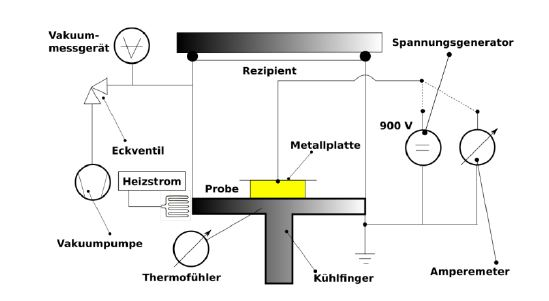
\includegraphics[width=0.9\textwidth]{abb/aufbau.JPG}
    \caption{Skizze des Rezipienten \cite{sample}}
    \label{abb:aufbau}
\end{figure}
Ist ein ausreichendes Vakkum im Rezipienten hergestellt wird der Plattenkondensator aufgeladen.
Durch das elektrische Felöd wird der Ionenkristall langsam polarisiert.
Daher sollte die Polarisationszeit wesentlich größer als die Relaxationszeit sein.
5 bis 10 Minuten sollten dafür ausreichend sein.
Nach der Polarisationszeit wird die Probe über den Kühlfinger auf $210$ Kelvin gekühlt.
Anschließend kann der Plattenkondensator ausgeschaltet werden,
da die Relaxationszeit jetzt verhältnismäßig groß ist.
Um Messfehler zu vermeiden wird der Plattenkondensator ca. 5 minuten Kurzgeschlussen, 
um ihn vollständig zu entladen.
Nun wird die Heizspannung wieder angelegt und so reguliert,
dass eine konstante Heizrate von $2 \frac{\text{Kelvin}}{\text{Minute}}$ bzw $1.5 \frac{\text{Kelvin}}{\text{Minute}}$ vorliegt.
Parallel wird der Strom am Kondensator mittels des Picoamperemeter gemessen.
Die Probe wird bis auf ca $330$ Kelvin erwärmt.
